\subsection{Bottleneck prevention}

\begin{figure}[htb!]
  \centering
    \subfloat[]{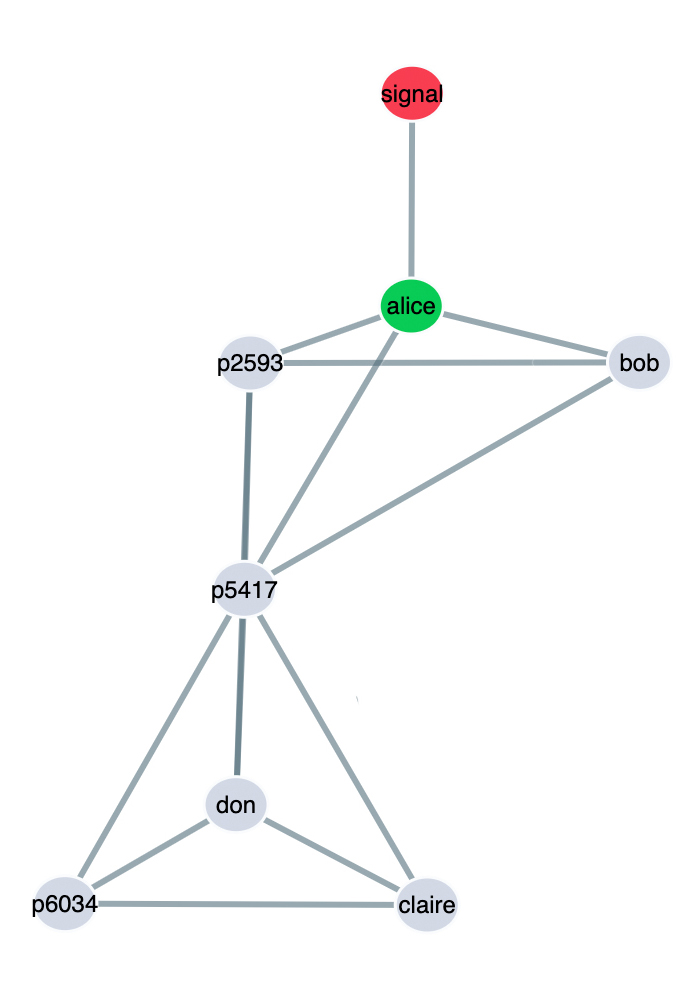
\includegraphics[width=0.33\textwidth]{graphics/analysis/mini-scenarios/bottleneck-prevention/1.jpg} \label{fig:filmstrips-bottleneck-prevention-a}}
    \subfloat[]{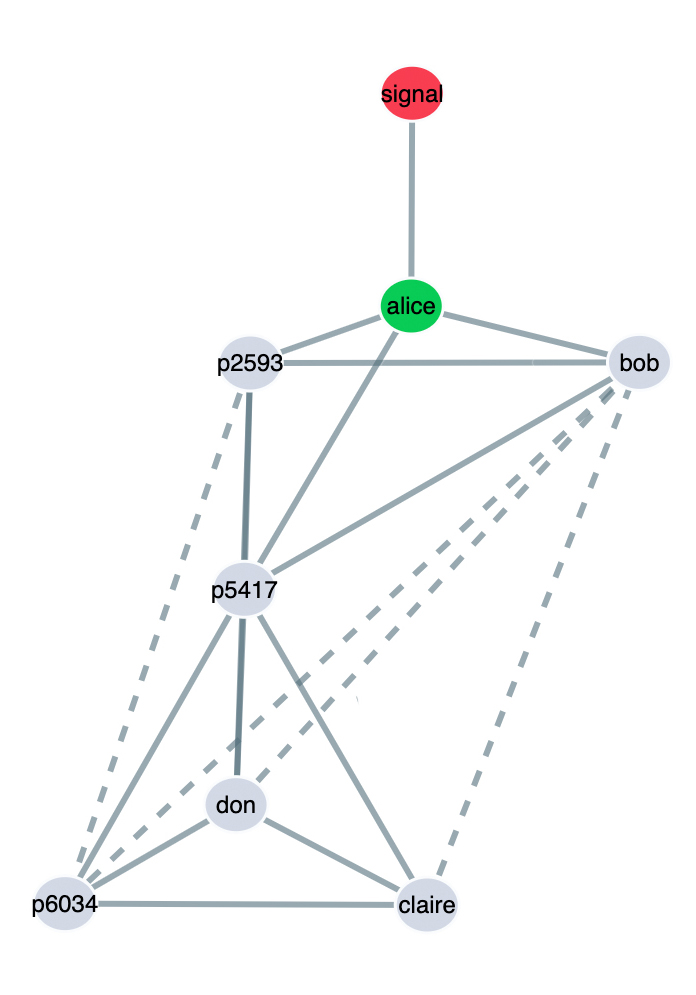
\includegraphics[width=0.33\textwidth]{graphics/analysis/mini-scenarios/bottleneck-prevention/2.jpg} \label{fig:filmstrips-bottleneck-prevention-b}}
	\subfloat[]{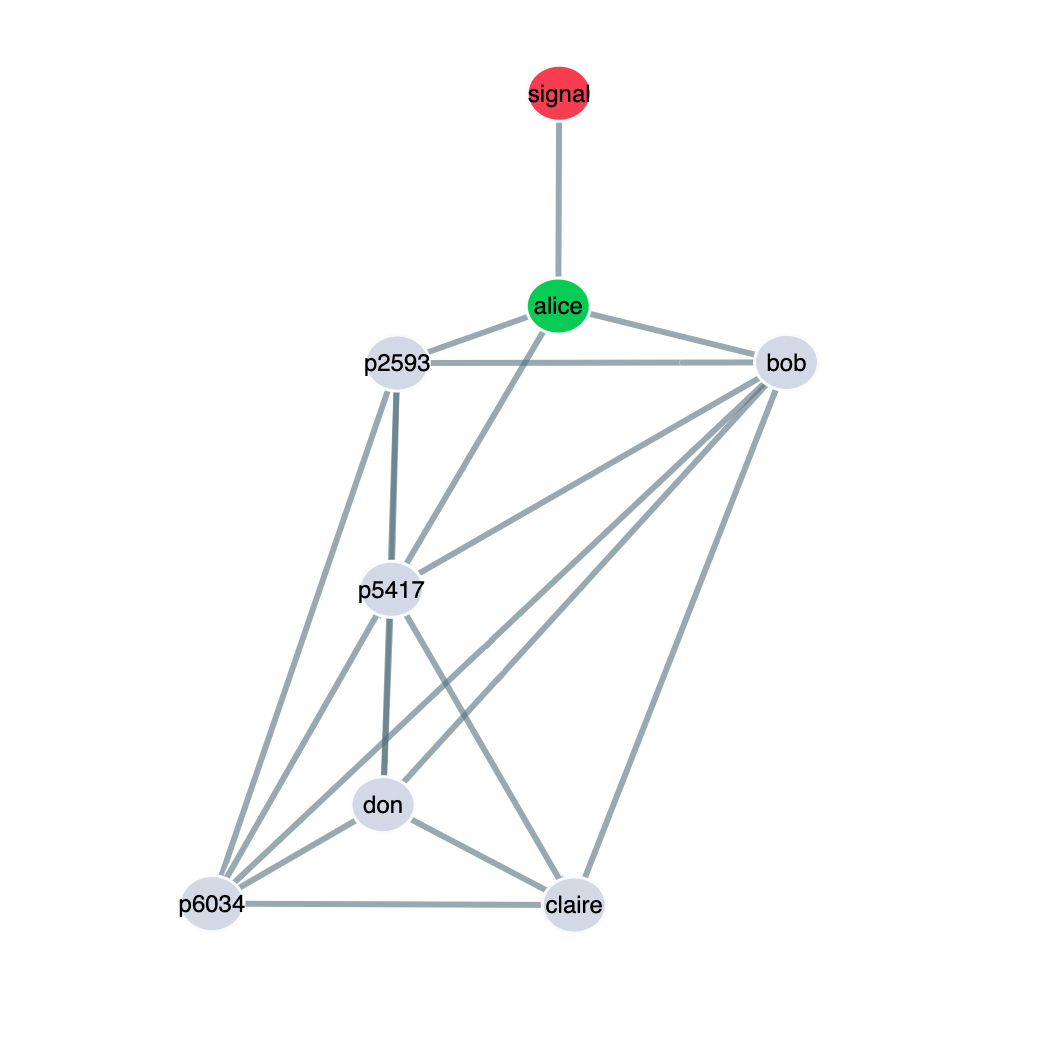
\includegraphics[width=0.33\textwidth]{graphics/analysis/mini-scenarios/bottleneck-prevention/3.jpg} \label{fig:filmstrips-bottleneck-prevention-c}}
	\caption{Preventing a bottleneck}
\label{fig:filmstrips-bottleneck-prevention}
\end{figure}

An important requirement of a network is that nodes can theoretically reach any other node in the network. This is guaranteed as long a path exists. In fact not only one path but multiple paths should exists to avoid critical nodes. A critical node is a node that others are dependent on to reach other nodes because its the node connecting two parts of the network. \vref{fig:filmstrips-bottleneck-prevention-a} shows a scenario where node \textit{p5417} connects two networks. In case it crashes or leaves the network, the other peers would be disconnected from the main network.

To mitigate critical nodes, Mitosis is introducing a \textit{Router-Gravity} metric. The Router-Gravity metric is used during the peer selecting process when a peer is acquiring new peers. A peer that is closer to the \router peer, thus delivering Router-Alive messages faster, is preferred in the selection over a peer that is not delivering messages at all. 
During the acquiring process a peer selects via peers from its directed connected peers to create new connections. The Via-Peers of a peer who is delivering the Router-Alive message faster are higher ranked then slower peers or peers that are not delivering the Router-Alive message at all.

\vref{fig:filmstrips-bottleneck-prevention-b} shows how the peers are connecting to the peers closer to the router. Thus they are creating new path to eliminate the critical node \textit{p5417} (\vref{fig:filmstrips-bottleneck-prevention-c}).
